\documentclass[fleqn,oneside,a4]{article}
\newcommand{\level}{\section}
\newcommand{\sublevel}{\subsection}
\newcommand{\subsublevel}{\subsubsection}
\hoffset = 0pt
\voffset = 0pt
\oddsidemargin = 0pt
\evensidemargin = 0pt
\topmargin = 0pt
\headsep = 0pt
\textheight = 600pt
\textwidth = 450pt

% \documentclass[fleqn,oneside,a4]{book}
% \newcommand{\level}{\chapter}
% \newcommand{\sublevel}{\section}
% \newcommand{\subsublevel}{\subsection}
% \usepackage[paperwidth=14.5cm, paperheight=21.5cm]{geometry}
% \hoffset = -35pt
% \voffset = -50pt
% \oddsidemargin = 0pt
% \evensidemargin = 0pt
% \topmargin = 0pt
% \textheight = 530pt
% \textwidth = 340pt

\usepackage{algorithm2e}
\usepackage{amsmath}
\usepackage{amsthm}
\usepackage{amssymb}
\usepackage{color}
\usepackage{dsfont}
\usepackage{enumitem}
\usepackage{graphicx}
\usepackage{hyperref}
\usepackage{listings}
\usepackage{mathtools}
\usepackage{makeidx}
\usepackage{multicol}
\usepackage{soul}
% \usepackage{tikz-cd}
\usepackage{wrapfig}

\hypersetup{
    colorlinks=false,
    pdfborder={0 0 0},
}

% Soft colors.

% \definecolor{red}{rgb}{0.8,0.1,0.1}
% \definecolor{blue}{rgb}{0.1,0.2,0.8}

% Some useful definitions.

\newcommand{\comment}[1]{\hl{#1}}
\newcommand{\la}{\leftarrow}
\newcommand{\Lra}{\Leftrightarrow}
\newcommand{\nat}{\mathds{N}}
\newcommand{\new}[1]{\textcolor{black}{#1}}  % blue
% \newcommand{\new}[1]{\fcolorbox{black}{white}{#1}}
\newcommand{\ol}{\overline}
\newcommand{\pcunchanged}{c_{t + 1} = c_t}
\newcommand{\Ra}{\Rightarrow}
\newcommand{\ra}{\rightarrow}
\newcommand{\term}[1]{\textit{#1}\index{#1}}
\newcommand{\altterm}[2]{\textit{#1}\index{#2}}
% \newcommand{\term}[1]{\textcolor{magenta}{#1}}
\newcommand{\true}{\textbf{true}}
\newcommand{\false}{\textbf{false}}

% Execution marks

\newcommand{\te}[1]{#1^T}      % Taint execution
\newcommand{\se}{\overline}    % Symbolic execution
\newcommand{\dse}{\widetilde}  % Dynamic symbolic execution

% Assert, declare and update as commands.

\newcommand{\assert}{\textbf{assert}\,}
\newcommand{\declare}{\textbf{declare}\,\,}
\newcommand{\update}{\textbf{update}\,\,}

% Assert, declare and update as statements.

% \newcommand{\assert}{c_{t + 1} = c_t \cup}
% \newcommand{\declare}{}
% \newcommand{\update}{}

\newcommand{\lblock}{ \left \{ \begin{array}{l} }
\newcommand{\rblock}{ \end{array} \right. }

\renewcommand{\arraystretch}{1.5}
% \renewcommand\qedsymbol{$\blacksquare$}

\newtheorem{theorem}{Theorem}
\newtheorem{lemma}[theorem]{Lemma}
\newtheorem{claim}{Claim}

\lstset{
    basicstyle=\linespread{0.9}\small\ttfamily,
    keywordstyle=\bfseries\color{black},
    stringstyle=\color{black},
    identifierstyle=\color{black}
}

\setlength{\parindent}{0em}

\title{Formal model of concrete, symbolic,
    dynamic symbolic execution (concolic execution),
    and taint tracking}
\author{Sergey Vartanov \\
    \href{mailto:me@enzet.ru}{\texttt{me@enzet.ru}},
    \href{mailto:svartanov@ispras.ru}{\texttt{svartanov@ispras.ru}}}
\makeindex

\begin{document}

\maketitle

\setlength{\parskip}{0em}

\tableofcontents

% \pagebreak

\setlength{\parskip}{0.5em}

\level{Concrete program execution}

The main goal of this document is to propose a formal definition of
some program analysis terms, such as execution (concrete execution),
(pure) symbolic execution,
dynamic symbolic execution (concolic execution),
feasibility, and taint analysis.

We want to propose as formal as possible definition of all terms we will use,


\sublevel{Program definition}

We will start with a program definition.
In order to separate program execution from
symbolic and dynamic symbolic execution, which will be discussed later,
we will use a term concrete program and concrete program execution
since it processes concrete data.

\subsublevel*{Knuth}

We can find classical definition of a \term{computational method} in
Donald Knuth's \textit{The Art of Computer Programming}~\cite{knuth}.
Computational method is $\langle Q, I, \Omega, f \rangle$,
where $f: Q \ra Q$, $Q$~--- states, $\Omega$~--- terminal states,
$I$~--- input states.

Execution:
$\forall x \in I$ path is $x_0, x_1, \dots, x_k, \dots$.
$x_0 = x, x_{k + 1} = f(x_k)$.

For the sake of convenience, we will use slightly different notation
because it will interfere with our further considerations:
$\mathcal{P} = \langle \mathcal{F}, D_I, D_T, D \rangle$,
where $\mathcal{F}: D \ra D$ is an \term{execution function},
$D$~--- states, $D_I$~--- initial states,
$D_T$~--- terminal states.

Without any doubts, any real-world program execution process can be described
by this definition.
% We can consider all accessible memory (including ) as $D$,

However, we want to highlight some particular aspects of modern programs and
computer systems.

\subsublevel*{Split execution function}

Firstly, execution function $\mathcal{F}$ is too complex.
It is a single function that manages the whole execution process.
To write a program we should

\altterm{Program}{program} is defined by functional elements and data:
    $\mathcal{P} = \langle F, F_I, F_T, D \rangle$,
where function elements and data are defined as follows:
\begin{itemize}
    \item $F = \{f_j\} = \{(f^F_j, f^D_j)\}$~is a \term{function element set}.
        $f_j: D \ra F \times D$~is a \term{function element}.
        $f_j = (f^F_j, f^D_j)$:
        \begin{itemize}
            \item $f^F_j: D \ra F$~is
                \term{control flow function element}.
            \item $f^D_j: D \ra D$~is \term{data flow function element}.
        \end{itemize}
        Function element could be considered as program instruction, that
        computes next program instruction \{$f^F_j$\}
        and modifies data \{$f^D_j$\}.
    \item $F_I$ is a set of \term{initial function elements}.
    \item $F_T$ is a set of \term{terminal function elements}.
    \item $D = \{d_j\}$ is a set of possible \term{data} values.
\end{itemize}

Additionally, we will assume the following.
\begin{itemize}
    \item Function element set is not empty: $F \neq \varnothing$.
    \item $\forall j \,\, f^F_j$ is a total function.
    \begin{itemize}
        \item If $f_j \notin F_T$,
            $\forall d \in D \,\, f^F_j(d) = f_k, f_k \in F$.
        \item If $f_j \in F_T$,
            $\forall d \in D \,\, f^F_j(d) = f_j$.
    \end{itemize}
    \item To simplify considering, we will assume that unless otherwise stated
        there is one and only one initial function element $f_0$:
        $F_I = \{f_0\}$.
    \item Program has at least one terminal function element:
        $F_T \neq \varnothing$.
\end{itemize}

\subsublevel*{Instruction counter}

We can assume, that there is a integer variable, that is a part of data
$i \in D$, that is \term{instruction counter}.
In this case, $f: D \ra D$, so
we have no $f_j^F$ component and $f_j = f^D_j$ only.

\subsublevel*{Limitations}

We assume \textbf{deterministic} program execution
using \textbf{limited} binary data without \textbf{self-modification}.
Concrete program execution means normal program execution on given binary data.

\begin{itemize}
    \item Firstly, we should emphasize that we distinguish data ($D$)
        from function elements ($F$).
        It implies that self-modification is not possible.
        To allow self-modification, we should merge $F$ and $D$ into one set.
    \item Program is deterministic: $f^F_j: D \ra F$.
        For nondeterministic program it should be: $f^F_j: D \ra F*$.
    \item Data is limited and predefined: $|D| < \infty$.
\end{itemize}

\subsublevel*{Possible data model definition}

Data set $D$ is a set of all possible values that can be arguments of
function elements $f_j$: $D = \{d_j\}$.
Data $d \in D$ is an abstract entity and it can be anything.
The simplest data definition is a set of values: $d = \{d^j\}, d \in D$
(we will use superscript for data elements because it is more convenient to use
subscript for data instances), where $d^j$ is a Boolean variable,
Boolean vector, natural, integer, real number, or anything else.

As we want to model real computer programs we can notice,
that simplest definition of data as a Boolean variables is useful enough
for majority of computer systems, which operates limited binary memory.

However it is convenient to use more complicated data definitions to simplify
modeling.

Binary data:
\begin{itemize}
    \item $B = (\false, \true), \mathcal{B}_2 = B^8$.
\end{itemize}

Data model definition with registers and memory:
\begin{itemize}
    \item $D_1 = \{d_j\} = R \cup M$.
    \begin{itemize}
        \item $R = \{r_j\}$~--- \term{concrete registers}.
            $r_j \in \mathcal{B}_2$.
        \item $M = \{m_j\}$~--- \term{concrete memory}. $m_j \in \mathcal{B}_2$.
    \end{itemize}
\end{itemize}

For the next data model definition we will
\textbf{avoid limited data condition}.
Here $Y$ is a set of sets $Y_i$.
Each set $Y_i$ may contain an arbitrary number of elements.
Data model definition with set of inputs, registers, memory,
and external knowledge about array allocation:
\begin{itemize}
    \item $D_2 = \{d_j\} = Y \cup R \cup M \cup L$. $|L| \le |M|$.
    \begin{itemize}
        \item $Y = \{Y_i\}$~--- \term{concrete inputs},
            $Y_i = \{y_{i, j}\}$~--- \term{concrete input}.
            $y_{i, j} \in \mathcal{B}_2$.
        % \item $Y = \{ Y_i \}$~--- \term{inputs},
        %     $Y_i = \langle \{y_{i, j}\}, y_{i, l} \rangle$~--- \term{input}.
        %     $y_{i, j} \in \mathcal{B}_2, y_{i, l} \in \mathcal{B}_2$.
        \item $R = \{r_j\}$~---
            \term{concrete registers}. $r_j \in \mathcal{B}_2$.
        \item $M = \{m_j\}$~---
            \term{concrete memory}. $m_j \in \mathcal{B}_2$.
        \item $L = \{l_j\}$~---
            \term{concrete array lengths}. $l_j \in \mathcal{B}_2$.
    \end{itemize}
\end{itemize}

\subsublevel*{Control flow graph}

Set of all possible next function elements for function element $f$ is
$f[D] = \{f_j \in F | f_j = f_j^F(d), d \in D\}$.
\altterm{Control flow graph}{control flow graph} is a directed graph where
vertices are function elements and there is an edge from
vertex $f_i$ to vertex $f_j$ iff $f_j \in f_i[D]$.
Function element $f_j = (f_j^F, f_j^D)$ is \term{branch} iff $|f_j[D]| > 1$.
Otherwise (if range of the control flow function
element has exactly one element),
function element is \term{operation},
i.e. iff $\exists f_k: f_j^D(d) = f_k, \forall d \in D$.

The set of all branches is $F_B = \{f_j \in F | |f_j[D]| > 1\}$.
The set of all operations is $F_O = \{f_j \in F | |f_j[D]| = 1\}$.
Since $|f_j[D]|$ by definition is either equals to 1, or greater than 1,
$F = F_B \cup F_O$ and $F_B \cap F_O = \varnothing$.

We will use graphical representation of control flow graph using circles
for vertices with function element captions and arrows for edges.
Vertices that correspond to terminal function elements will be represented
by circles with double stroke.
Vertices that correspond to initial function elements will be represented
as usual.
We assume that either there is a single initial element $f_0$,
or initial elements are represented by vertices that has no incoming edges.

\altterm{Basic blocks}{basic block} are sets of \comment{continue...}

\subsublevel*{Semantics}

\begin{wraptable}{r}{6cm}
    \begin{center}
        \begin{tabular}{| c | c |}
            \hline
            $(x, y)$         & $f^D_\land(x, y)$ \\ \hline \hline
            (\false, \false) & (\false, \true)   \\ \hline
            (\false, \true)  & (\false, \true)   \\ \hline
            (\true, \false)  & (\false, \true)   \\ \hline
            (\true, \true)   & (\true, \true)    \\ \hline
        \end{tabular}
        \label{tbl:conjunction}
    \end{center}
    \caption{Conjunction truth table.}
\end{wraptable}

\altterm{Concrete semantics}{concrete semantics} is a set of all data function
elements $f^D_j$ used in program: $F^D$.
In other words, concrete semantics defines
possible ways to transform data in program.
It could be considered as an instruction set, or a system of commands.

Semantics cannot be defined without data $D$ definition.
For example, let's take a look at logical conjunction.
It is a binary logical operator, which means it uses two Boolean operands
and returns Boolean result.
But to define an operation $f^D_\land$, that performs logical conjunction,
we should also define data $D$ and how this operation transform data.
Let's define its semantics as $f^D_\land(x, y) = (x \land y, y)$,
where $x, y \in B$.
It could be represented in the form of assignment $x \la x \land y$.
It could also be represented in the form of truth table
(see Table \ref{tbl:conjunction}).

\sublevel{Execution}

We consider that program execution is an iterative process with steps.
For further considerations we will use variable $t \in \nat$ as
\term{execution step}.
At every step program execution has its \term{program state} $s = (f, d)$:
next function element (next instruction) and current \term{data state}.
$f \in F, d \in D$.
Set of all possible execution states is $S$.
Program state at the iteration $t$ is
$s_t = (f_t, d_t) = \big((f_t^F, f_t^D), d_t\big)$.
$(f_0, d_0), f_0 \in F_I$ is \term{initial state}.
Any state $(f_t, d_t)$ such as $f_t \in F_T$ is \term{terminal state}.

We consider that there is \term{execution function} $\mathcal{F}: S \ra S$
that manages the execution process:
\[\mathcal{F}(s_t) = \mathcal{F}\big((f_t, d_t)\big) =
    f_t(d_t) =
    \big(f_t^F(d_t), f_t^D(d_t)\big) =
    (f_{t + 1}, d_{t + 1}) = s_{t + 1}.\]

Execution function $\mathcal{F}$ defines an \term{execution rule}:
\begin{itemize}
    \item $f_{t + 1} = f_t^F(d_t)$,
    \item $d_{t + 1} = f_t^D(d_t)$.
\end{itemize}

\altterm{Execution of a program}{program execution}
$\mathcal{P} = \langle F, F_I, F_T, D \rangle$
on \term{input data} $d_0$, where $F_I = \{f_0\}$,
is a chain of program states,
starting with initial state $s_0 = (f_0, d_0)$,
where next state is a function $\mathcal{F}$ of previous state:
$s_{t + 1} = \mathcal{F}(s_t), s_t \in S$.
Therefore execution can be represented as iterative use of execution function:
$\mathcal{F}(\mathcal{F}(\dots\mathcal{F}(d_0)\dots))$.

We consider that if program execution approaches state $s_t = (f_t, d_t)$,
where $f_t \in F_T$, program execution is terminated.
Hence, execution is either infinite chain
\[E(d_0) = s_0 \ra s_1 \ra \cdots \ra s_t \ra \cdots =
        (f_0, d_0) \ra (f_1, d_1) \ra \cdots \ra (f_t, d_t) \ra \cdots,\]
where $\forall j \,\, f_j \notin F_T$ (in this case $d_t$ is an
\term{output data} of program execution $E(d_0)$),
or finite chain
\[E(d_0) = s_0 \ra s_1 \ra \cdots \ra s_t =
        (f_0, d_0) \ra (f_1, d_1) \ra \cdots \ra (f_t, d_t),\]
where $f_t \in F_T \land \forall j < t \,\, f_j \notin F_T$
(in this case execution has no output data).
For the first case we will use notation $E(d_0) \ra d_t$,
for the second: $E(d_0) \ra \infty$.

Note, that execution is a sequence of states:
$E(d_0) = (s_0, s_1, \dots, s_t, \dots)$.
But we will use notation
$E(d_0) = s_0 \ra s_1 \ra \dots \ra s_t \ra \dots$
to emphasize that it is a process.

\begin{lemma}
    \label{exists_one_execution}
    $\forall \mathcal{P} = \langle F, F_I, F_T, D \rangle \,\,
    \forall d \in D \,\, \exists! E(d)$.
\end{lemma}

\begin{proof}
    Let's prove it by constructing the execution chain.
    By the program definition, there is a initial function element $f_0$.
    Hence, $\forall d \in D$
    there is a initial program state $s_0 = (f_0, d)$.
    For every program state $s_t = (f_t, d_t)$,
    either $f_t \notin F_T \Ra f_t(d_t) = (f_{t + 1}, d_{t + 1})$
        and we have next step of the execution,
    or $f_t \in F_T \Ra$ execution is terminated.
    All steps of this process are deterministic,
    hence we will have execution $E(d)$ determined by initial input data $d$.
\end{proof}

To visualize the process of the program execution we will use circles
for program states connected by arrows which depicts function $\mathcal{F}$.
If program execution is finite, the last state will be depicted by
a circle with double stroke.

\begin{figure}[h!]
    \begin{center}
        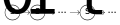
\includegraphics[scale=1.25]{pdf/concrete_execution.pdf}
    \end{center}
    \caption{Infinite and finite concrete program execution}
\end{figure}

We will also define \term{execution path} as either any finite sequence
$P = (f_0, f_1, \dots, f_t)$, where
$\forall j \,\, f_j \in F \land f_{j + 1} \in f_j[D]$
and $f_t \in F_T \land \forall j < t \,\, f_j \notin F_T$
or infinite sequence $P = (f_0, f_1, \dots, f_t, \dots)$, where
$\forall j \,\, f_j \in F \land f_{j + 1} \in f_j[D] \land f_j \notin F_T$.

\begin{lemma}
    There is one and only one execution path $P$ for the execution $E(d_0)$.
    \[ \begin{array}{c}
    \forall E(d_0) = s_0 \ra s_1 \ra \cdots \ra s_t \ra \cdots =
        (f_0, d_0) \ra (f_1, d_1) \ra \cdots \ra (f_t, d_t) \ra \cdots \\
    \exists! P = (f'_0, f'_1, \dots, f'_t, \dots):
        f'_0 = f_0, f'_1 = f_1, \dots, f'_t = f_t, \dots
    \end{array} \]
\end{lemma}

\begin{proof}
    Let's create a sequence $P = (f_0, f_1, \dots, f_t, \dots)$ from
    execution states.
    Now we have to proof that $P$ is execution path.
    Choose arbitrary $f_j = (f_j^F, f_j^D)$ and $f_{j + 1}$.
    By execution definition,
    $f_{j + 1} = f_j^F(d_j) \Ra f_{j + 1} \in f_j[D]$.
    Hence, $P$ is an execution path.
\end{proof}

We will denote this fact as $E(d_0) \Ra P$.

Let's also define a \term{branch chain} $P_B$ of a execution path $P$
as a subsequence of $P$, which contains only $f_j \in F_B$.
We can denote this fact as $P \Ra P_B$.

% $P_B = \{f_{j_0}, f_{j_1}, \dots, f_{j_k}, \dots\}$, where
% $\forall k \,\, f_{j_k} \in F_B$

\begin{lemma}
    $\forall P_B \,\, \exists! P: P \Ra P_B$.
\end{lemma}

\begin{proof}
    \comment{Add proof.}
\end{proof}

Therefore, we can write $P \Lra P_B$.

Note, that we define execution path just as a path in control flow graph.
It could be infeasible if there is no such input data that implies that path.
Execution path $P$ is \term{feasible in concrete model} iff
$\exists d_0 \in D: (f_1, d_1) = f_0(d_0) \land
    \forall j > 0 ~ (f_j, d_j) = f_{j - 1}(d_{j - 1})$.

Some sets of program executions:
\begin{itemize}
    \item $\mathds{E}_\mathcal{P}$~--- set of all possible program executions.
    \item $\mathds{P}_\mathcal{P}$~--- set of all possible execution paths.
        $\mathds{P}'_\mathcal{P}$~---
        set of all possible feasible execution paths.
\end{itemize}

\subsublevel*{Number of paths}

\begin{lemma}
    $|\mathds{E}_\mathcal{P}| = |D| |\mathcal{B}|$.
\end{lemma}

\begin{proof}
    $|D| |\mathcal{B}|$~--- number of all possible data states.
    From lemma \ref{exists_one_execution},
        $\forall d \in D \,\, \exists! E(d)$.
    $\forall d', d'' \in D : d' \neq d'' \,\, E(d') = (f_0, d') \ra \cdots
        E(d'') = (f_0, d'') \ra \cdots.
        (f_0, d') \neq (f_0, d'') \Ra E(d') \neq E(d'').$
    Therefore, number of possible executions is equal to number of
    possible initial input data.
\end{proof}

\begin{lemma}
    $|\mathds{P}''_\mathcal{P}| \le |D| |\mathcal{B}|$.
\end{lemma}

\level{Symbolic execution model}

Symbolic execution of the program is
an execution of a symbolic model of that program.
Symbolic model includes a set of symbolic function element
(symbolic models of function elements) and
symbolic data model.
Execution is performed using symbolic variables instead of concrete data.

\sublevel{Model}

$\se{\mathcal{P}} = \langle \se{F}, \se{F}_I, \se{F}_T, \se{D} \rangle$
is a \term{symbolic model} of program
$\mathcal{P} = \langle F, F_I, F_T, D \rangle$.
There are a lot of ways to create a symbolic model of a program,
therefore we will use some particular set of rules $R_\text{SE}$.
We can write it as
$\mathcal{P} \xrightarrow[]{R_\text{SE}} \se{\mathcal{P}}$.
It denotes that for all $\mathcal{P}$ exists only one symbolic model
$\se{\mathcal{P}}$ constructed using the set of rules $R_\text{SE}$.

Function elements and data is defines as follows.
\begin{itemize}
    \item $\se{F} = \{\se{f}_j\} =
        \{(\se{f}_j^F, \se{f}_j^D, \se{f}_j^C)\}$~---
        \term{symbolic function element models}
        that correspond to function elements of the program $\mathcal{P}$.
    \item $\se{F}_I$ is a set of
        \term{initial symbolic function element models},
        that correspond to initial function elements
        of the program $\mathcal{P}$.
    \item $\se{F}_T$ is a set of
        \term{terminal symbolic function element models},
        that correspond to terminal function elements
        of the program $\mathcal{P}$.
    \item $\se{f}_j: \se{D} \times C \ra
        (\se{F} \times \se{D} \times C)*$~---
        \term{symbolic function element model}.
    % %%% Not sure we have to divide function $\se{f}_j$.
    % \begin{itemize}
    %     \item $\se{f}_j^F: \varnothing \ra \se{F}*$~---
    %         \term{control flow symbolic function element model},
    %     \item $\se{f}_j^D: \se{D} \ra \se{D}*$~---
    %         \term{data symbolic function element model}.
    %     \item $\se{f}_j^C: \se{D} \times C \ra C*$~---
    %         \term{data symbolic function element model}.
    % \end{itemize}
    % \end{itemize}
\end{itemize}

\subsublevel*{Data model}

Symbolic data model $\se{D}$ is a symbolic model of program data $D$:
$D \xrightarrow[]{R_\text{SE}} \se{D}$.
To build a symbolic data model $\se{D}$ of a program, we should choose,
which items of the original data $D$ to be symbolized.
Let's assume out original data $D$ is a set of elements ($D = \{d_j\}$)
and we want to symbolize all of them in our model.

Firstly, we have to define a set of
\altterm{symbolic variables}{symbolic variable}
as a set of variables $X = \{x_j\}$.
And let symbolic data model $\se{D}$ be a

Data model with memory, registers, and array lengths.

\begin{itemize}
    \item $\se{D} = \{\se{d}_j\} = \se{R} \cup \new{\se{M}} \cup \se{L}$~---
        \term{symbolic data model}.
        \begin{itemize}
            \item $\se{R} = \{\se{r}_j\}, \se{r}_j = x_r, x_r \in X_R$~---
                \term{symbolic registers model}.
            \item $\se{M} = \{\se{m}_j\}, \se{m}_j = x_m, x_m \in X_M$~---
                \term{symbolic memory model}.
            \item $\se{L} = \{\se{l}_j\}, \se{l}_j = x_l, x_l \in X_L$~---
                \term{symbolic length model}.
        \end{itemize}
    \item $X = X_M \cup \new{X_L} \cup X_R$.
        \begin{itemize}
            \item $X_M = \{x_m\}$~---
                \term{memory symbolic variables}. $x_m \in \mathcal{B}$.
            \item \new{$X_L = \{x_l\}$~--- \term{length symbolic variables}.
                $x_l \in \mathcal{B}$.}
            \item $X_R = \{x_r\}$~---
                \term{register symbolic variables}. $x_r \in \mathcal{B}$.
        \end{itemize}
\end{itemize}

\comment{We don't consider data element indices as entities.
That's why they cannot be represented by symbolic variables (or can they?).
There should be such a data model.}

\subsublevel*{Path condition}

Set $C$ is called \term{path condition} or \term{path constraint}.
It is a logical expression over Boolean variables
$X = \{x_k\}, x_k \in \mathcal{B}$ called
\altterm{symbolic variables}{symbolic variable}.

\subsublevel*{Symbolic function element models}

Symbolic function element models are constructed from function elements of the
original program:
$F \xrightarrow[]{R_\text{SE}} \se{F}$, and
$\forall j \,\, f_j \xrightarrow[]{R_\text{SE}} \se{f}_j$.

\[ \se{f}_t(d_t, c_t) =
    \begin{cases}
        (\se{f}, \se{d}, c), \\
        (\se{f}, \se{d}, c), \\
        \dots \\
        (\se{f}, \se{d}, c).
    \end{cases} \]

Symbolic function element models are multivalued functions.
Number of values for each $\se{f}_j$ is predefined and doesn't depend on
its arguments.

\sublevel{Execution}

Symbolic execution unlike concrete execution is not an iterative process.
However, it has execution states
$\se{s} = (\se{f}, \se{d}, c)$~--- \term{symbolic state},
$\se{f} \in \se{F}, \se{d} \in \se{D}, c \in C$.
Set of all possible symbolic states is $\se{S}$.
$(\se{f}_0, \se{d}_0, \true)$ is an \term{initial symbolic state}.
Any state $(\se{f}_t, \se{d}_t, c_t)$, such as $\se{f}_t \in \se{F}_T$
is a \term{symbolic terminal state}.
Note, that $t$ is not an execution step here, but a state identifier.

We consider that there is a \term{symbolic execution function}
$\se{\mathcal{F}}: \se{S} \ra \se{S}$
that manages the symbolic execution process:

\begin{align*}
\se{\mathcal{F}}(s_{k, \dots, l})
&= \se{\mathcal{F}}
    \big((f_{k, \dots, l}, d_{k, \dots, l}, c_{k, \dots, l})\big) = \\
&= \big((f_{k, \dots, l, m}, d_{k, \dots, l, m}, c_{k, \dots, l, m}), \dots, 
       (f_{k, \dots, l, n}, d_{k, \dots, l, n}, c_{k, \dots, l, n})\big) = \\
&= (s_{k, \dots, l, m}, \dots, s_{k, \dots, l, n})
\end{align*}

\altterm{Symbolic execution}{symbolic execution}
$\se{E} = \se{s}_0 \ra \cdots$ visualization is
presented on Figure \ref{img:symbolic_execution}.

% \begin{tikzcd}
%     && \se{s}_{0,0,0} \arrow{r} & \cdots \\
%     & \se{s}_{0,0} \arrow{ru} \arrow{r} \arrow{rd} & \cdots \\
%     \se{E} = \se{s}_0 \arrow{r} \arrow{ru} \arrow{rd} & \cdots & 
%         \se{s}_{0,0,n_{0,0}}
%         \arrow{r} & \cdots \\
%     & \se{s}_{0,n_0} \arrow{r} & \cdots
% \end{tikzcd}

\begin{figure}[h!]
    \begin{center}
        \includegraphics[scale=1.25]{pdf/symbolic_execution.pdf}
    \end{center}
    \caption{Symbolic execution process.}
    \label{img:symbolic_execution}
\end{figure}

Execution rule:
\begin{itemize}
    \item $\{\se{f}_{0, t_1, \dots, t_n, 0}, \dots,
            \se{f}_{0, t_1, \dots, t_n, m}\} =
        \se{f}_{0, t_1, \dots, t_n}^F(\se{d}_{0, t_1, \dots, t_n})$,
    \item $\{\se{d}_{0, t_1, \dots, t_n, 0}, \dots,
            \se{d}_{0, t_1, \dots, t_n, m}\} =
        \se{f}_{0, t_1, \dots, t_n}^D(\se{d}_{0, t_1, \dots, t_n})$.
\end{itemize}

Execution path $P = \{\se{f}_0, \se{f}_1, \dots, \se{f}_t\}$ is
\term{feasible in symbolic model} iff $c_{0, 1, \dots, t}$ is true.

 \comment{Difference between forward and backward symbolic execution?
What is exactly backward symbolic execution?}

\sublevel{Symbolic semantics}

The major part of symbolic program model is a symbolic semantics.
We should define symbolic semantics for each function element from the original
program.

\sublevel{Symbolic execution and concrete execution}

 \comment{Feasibility in concrete model vs feasibility in symbolic model.}

\sublevel{Static symbolic execution}

 \comment{Some thoughts goes here.}

\level{Taint tracking}

\altterm{Taint tracking}{taint tracking} is a technique used to track data
flow in program during its execution.
To use taint tracking we should define a set that will be used to mark data
elements, initial taint marks distribution (or taint sources),
and taint policy---rules that describes taint propagation.

\sublevel{Model}

The set of a possible taint marks will be denote as $\mathcal{T}$.
Simplest useful taint set is $B = \{\false, \true\}$,
that divides data elements into two disjoint sets:
what is tainted and what is not.

\altterm{Taint data model}{taint data model} is
$\te{D} = \{\te{d}_j\}, \te{d}_j \in \mathcal{T}$.

Taint semantics is called \term{taint policy}.

\subsublevel*{Possible data model definitions}

If original data model consists of memory and registers $D = (M, R)$,
taint data model could be defined as $\te{D} = (\te{M}, \te{R})$:

\begin{itemize}
    \item $\te{M} = \{\te{m}_j\}, \te{m}_j \in \mathcal{T}$~---
        \term{taint memory model},
    \item $\te{R} = \{\te{r}_j\}, \te{r}_j \in \mathcal{T}$~---
        \term{taint registers model}.
\end{itemize}

 \comment{Definitions of undertainting and overtainting.}

\level{Dynamic symbolic (concolic) execution model}

Dynamic symbolic execution or, in other words, concolic execution,
is an execution of a program along with execution of its symbolic model
(that means construction of a path condition) but for the particular
execution path that is defined by initial input data $d_0$.

\sublevel{Model}

Model for dynamic symbolic execution consists of program model
$\mathcal{P} = \langle F, F_I, F_T, D \rangle$ and its symbolic model
$\se{\mathcal{P}} = \langle \se{F}, \se{F}_I, \se{F}_T, \se{D} \rangle$.
Dynamic symbolic execution program model could we presented as
\[\dse{\mathcal{P}} = \langle F, F_I, F_T, D,
\se{F}, \se{F}_I, \se{F}_T, \se{D} \rangle.\]

\begin{itemize}
        \item $Y = \{Y_i\}$~--- \term{taint sources}.
              $Y_i = (\{y_{i_j}\}, \new{y_{i_L}})$,
              $y_{i_j} \in \mathcal{B}$~--- \term{taint source elements},
              \new{$y_{i_L} \in \mathcal{B}$~--- \term{taint source size}}.
\end{itemize}

\sublevel{Execution}

As a concrete execution, it is iterative process with steps.
We will also use variable $t \in \nat$ as execution step.
At every step, there are program execution state $s_t = (f_t, d_t)$
and symbolic execution state $\se{s}_t = (\se{f}_t, \se{d}_t, c_t)$,
which we combine into \term{concolic state}
$\dse{s}_t = (f_t, d_t, \se{f}_t, \se{d}_t, c_t)$.

We consider that there is dynamic symbolic execution function
$\dse{\mathcal{F}}: \dse{S} \ra \dse{S}$
that manages the execution process:
\begin{align*}
\dse{\mathcal{F}}(\dse{s}_t) &=
    \dse{\mathcal{F}}\big((f_t, d_t, \se{f}_t, \se{d}_t, c_t)\big) = \\
    &= (f_t^F(d_t), f_t^D(d_t),
        \se{f}_t^F(\se{d_t}), \se{f}_t^D(\se{d_t}), c_{t + 1}) = \\
    &= (f_{t + 1}, d_{t + 1}, \se{f}_{t + 1}, \se{d}_{t + 1}, c_{t + 1}) = \\
    &= \dse{s}_{t + 1}.
\end{align*}

$c_{t + 1} = c_t \land e_t$.

We will define $e_t$ as follows.

If $f_t$ is an operation ($f_t \in F_O \Ra f_{t + 1} = \text{const}$):

% \begin{align*}
%     & \forall d', d'' \in D \,\, \\
%     & f_t^D(d') = d'' \Ra e_t \bigg\rvert_{\substack{
%         \se{d}^0_t = d'^0, \se{d}^0_{t + 1} = d''^0 \\
%         \dots \\
%         \se{d}^n_t = d'^n, \se{d}^n_{t + 1} = d''^n
%     }} = \true \\
%     & f_t^D(d') \neq d'' \Ra e_t \bigg\rvert_{\substack{
%         \se{d}^0_t = d'^0, \se{d}^0_{t + 1} = d''^0 \\
%         \dots \\
%         \se{d}^n_t = d'^n, \se{d}^n_{t + 1} = d''^n
%     }} = \false \\
% \end{align*}

\begin{align*}
    & \forall d', d'' \in D \,\, \\
    & f_t^D(d') = d'' \Ra e_t \bigg\rvert_{
        \, \se{d}_t = d', \se{d}_{t + 1} = d''} = \true \\
    & f_t^D(d') \neq d'' \Ra e_t \bigg\rvert_{
        \, \se{d}_t = d', \se{d}_{t + 1} = d''} = \false \\
\end{align*}

If $f_t$ is a branch
($df_t \in F_B \Ra _{t + 1} = d_t, f_{t + 1} = f' or f ''$):

\begin{align*}
    & \forall d', \in D \,\, \\
    & f_t^D(d') = d'' \Ra e_t \bigg\rvert_{
        \, \se{d}_t = d', \se{d}_{t + 1} = d'} = \true \\
    & f_t^D(d') \neq d'' \Ra e_t \bigg\rvert_{
        \, \se{d}_t = d', \se{d}_{t + 1} = d'} = \false \\
\end{align*}

Execution function $\dse{\mathcal{F}}$ defines an \term{execution rule}:
\begin{itemize}
    \item $f_{t + 1} = f_t^F(d_t)$,
    \item $d_{t + 1} = f_t^D(d_t)$,
    \item $\se{f}_{t + 1} = \comment{?}$,
    \item $\se{d}_{t + 1} = \comment{?}$,
    \item $c_{t + 1} = \comment{?}$.
\end{itemize}

\altterm{Dynamic symbolic execution}{dynamic symbolic execution}
(or \term{concolic execution})
of a program $\mathcal{P} = \langle F, F_I, F_T, D \rangle$
and a symbolic model
$\se{\mathcal{P}} = \langle \se{F}, \se{F_I}, \se{F_T}, \se{D} \rangle$
is a chain of concolic states, starting with initial state
$\dse{s}_0 = (f_0, d_0, \se{f}_0, \se{d}_0, \true)$,
where the next state is a function $\dse{\mathcal{F}}$ of previous state:
\[s_{t + 1} = (f_{t + 1}, d_{t + 1}) = (f_t^F(d_t), f_t^D(d_t)) =
    \dse{\mathcal{F}}(s_t), s_t \in S\]

$\dse{E}(d_0) = \dse{s}_0 \ra \dse{s}_1 \ra \dots \ra \dse{s}_t \ra \dots$.

\sublevel{Path alternation}

\altterm{Path alternation}{path alternation}is a technique
to construct new execution paths using dynamic symbolic execution.
Assume, that we have dynamic symbolic execution path
$\dse{E}(d_0) = \dse{s}_0 \ra \dse{s}_1 \ra \dots \ra \dse{s}_t \ra \dots$.
There are states that we will call \altterm{branch states}{branch state}:
$\dse{S}_B = \{\dse{s}_t = (f_t, d_t, \se{f}_t, \se{d}_t, c_t) :
f_t \in F_B\}$.
For each branch state we can try to perform path alternation.

Consider we have chose a branch state
$\dse{s}_t = (f_t, d_t, \se{f}_t, \se{d}_t, c_t) \in \dse{S}_B$.
As it is a branch state, $f_t \in F_B$.
Hence, $|f_t[D]| > 1$.
Suppose, $f_t(d_t) = f_u \Ra \exists f_v \neq f_u: f_v \in f_t[D]$.

$(c_0, c_1, \dots, c_t), c_0 = \true$.

$\forall j = \ol{1, t} \,\, c_j = e_0 \land e_1 \land \dots \land e_j$.

$c_t = e_0 \land e_1 \land \dots \land e_t$.

$c*_t = e_0 \land e_1 \land \dots \land \ol{e_t}$.

\begin{lemma}
    If $\exists d': c*_t(d')$,
    $\dse{E}(d') = (s'_0, s'_1, \dots, s'_t, \dots),
    s'_t = (f_t, d'_t, \se{f}'_t, \se{d}'_t, c'_t),
    f_t(d'_t) = f_v \neq f_u$.
\end{lemma}

 \comment{Divergence?}

 \comment{Selective symbolic execution.}

\level{Examples}

In that section we will consider some primitive programs
to research their properties.

\sublevel{Simplest program}

\subsublevel*{Definition}

Simplest program that performs some logical binary operation $\diamond$
of two Boolean variables: $x \la x \diamond y$ looks like:
\begin{itemize}
    \item $\mathcal{P}_{\diamond} = \langle F, F_I, F_T, D \rangle =
        \langle \{f_0, f_1\}, \{f_0\}, \{f_1\}, \{x, y\} \rangle$,
    \item $x, y \in \mathcal{B} = \{\false, \true\}$,
    \item $f_0 = (f^F_0, f^D_0), f^F_0(\{x, y\}) = f_1,
        f^D_0(\{x, y\}) = \{x \diamond y, y\}$.
    \item $f_1 = (f^F_1, f^D_1), f^F_1(\{x, y\}) = f_1,
        f^D_1(\{x, y\}) = \{x, y\}$.
\end{itemize}

\begin{figure}[h!]
    \begin{center}
        \includegraphics[scale=1.25]{pdf/simple.pdf}
    \end{center}
    \caption{Control flow graph, execution paths,
        and symbolic execution tree of a simple program.}
\end{figure}

\subsublevel*{Properties}

Since the program has no branches, symbolic execution tree is the same as
control flow graph and there is only one execution path.
Since its data contains only two Boolean variables,
there are 4 possible executions.
For example, if operation $\diamond$ is logical and ($\land$):

\begin{itemize}
    \item $E(\false, \false) \ra (\false, \false),$
    \item $E(\false, \true) \ra (\false, \true),$
    \item $E(\true, \false) \ra (\false, \false),$
    \item $E(\true, \true) \ra (\true, \true).$
\end{itemize}

We can write a static symbolic execution formula of this program:
\[(x, y) \ra (x \diamond y, y)\]

\sublevel{Simplest branch program}

\subsublevel*{Definition}

Simplest program that contains branch:
\begin{itemize}
    \item $\mathcal{P}_{\text{branch}} = \langle F, F_I, F_T, D \rangle =
        \langle \{f_0, f_1, f_2\}, \{f_0\}, \{f_1, f_2\}, D \rangle$,
    \item $f_0^F[D] = \{f_1, f_2\}$,
        $f_1^F[D] = \{f_1\}$, $f_2^F[D] = \{f_2\}$.
\end{itemize}

\begin{figure}[h!]
    \begin{center}
        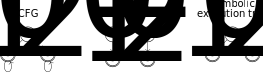
\includegraphics[scale=1.25]{pdf/execution_branch.pdf}
    \end{center}
    \caption{Control flow graph, execution paths,
        and symbolic execution tree of a program with one branch.}
\end{figure}

\subsublevel*{Properties}

$|\mathds{P}_\mathcal{P}| = 2$.
$1 \le |\mathds{P}''_\mathcal{P}| \le 2$.

\sublevel{Simplest cycle program}

\subsublevel*{Definition}

Simplest program that contains a cycle:
\begin{itemize}
    \item $\mathcal{P}_{\text{cycle}} = \langle F, F_I, F_T, D \rangle =
        \langle \{f_0, f_1, f_2\}, \{f_0\}, \{f_1\}, D \rangle$,
    \item $f_0^F[D] = \{f_0, f_1\}$. $f_1^F[D] = \{f_1\}$.
\end{itemize}

\begin{figure}[h!]
    \begin{center}
        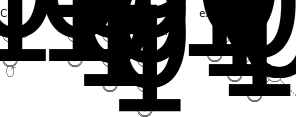
\includegraphics[scale=1.25]{pdf/execution_cycle.pdf}
    \end{center}
    \caption{Control flow graph, execution paths,
        and symbolic execution tree of a program with one cycle.}
\end{figure}

\subsublevel*{Properties}

$|\mathds{P}_\mathcal{P}| = \infty$.
$1 \le |\mathds{P}''_\mathcal{P}|$.

\sublevel{Change data under tainted condition}

\subsublevel*{Code snippet}

\lstset{language=c,caption=Listing,label={lst:impl}}
\begin{lstlisting}[numbers=left,numberstyle=\scriptsize]
int x = read();
int y;

if (x == 1) {
    y = 1;
} else {
    y = 2;
}
y += 1;
\end{lstlisting}

\subsublevel*{Definition}

We can formalize it as follows.
\begin{itemize}
    \item $\mathcal{P}_\text{IF} = \langle F, F_I, F_T, D \rangle =
    \langle \{f_0, f_1, f_2, f_3, f_4, f_5\},
        \{f_0\}, \{f_5\}, \{x, y\} \rangle$,
    \item $x, y \in \mathcal{B} = \{\false, \true\}$,
    % \item $f_0 = (f^F_0, f^D_0), f^F_0(\{x, y\}) = f_1,
    %     f^D_0(\{x, y\}) = \{x \diamond y, y\}$.
    % \item $f_1 = (f^F_1, f^D_1), f^F_1(\{x, y\}) = f_1,
    %     f^D_1(\{x, y\}) = \{x, y\}$.
\end{itemize}

\begin{figure}[h!]
    \begin{center}
        \includegraphics[scale=1.25]{pdf/implicit.pdf}
    \end{center}
    \caption{Implicit flow program control flow graph}
\end{figure}

\sublevel{Table values}

\subsublevel*{Code snippet}

 \comment{For this one we should have memory indexing.
How can we reach that?}

\lstset{language=c,caption=Listing,label={lst:impl}}
\begin{lstlisting}[numbers=left,numberstyle=\scriptsize]
char* a = read_array();
char* b = init_array();
char* map = {"a...zA...Z"};

for (int i = 0; i < a.length(); i++) {
    if (a[i] > 26) {
        b[i] = map[a[i] - 'a' - 26]
    } else {
        b[i] = a[i];
    }
}
\end{lstlisting}

 \comment{It is just write by tainted index.}

\sublevel{Sequence comparison}

Code example, in which program compare input string with some
predefined string constant, could be considered as a classic example.
Variations of this example can be found in papers describes
dynamic symbolic execution tools.

Example from SAGE paper~\cite{sage}: compare input string of 4 bytes length
with string constant \texttt{"bad!"}, if it so, trigger an error state.
\lstset{language=c,caption=Listing,label={lst:sage}}
\begin{lstlisting}[numbers=left,numberstyle=\scriptsize]
void top(char input[4]) {
    int cnt=0;
    if (input[0] == 'b') cnt++;
    if (input[1] == 'a') cnt++;
    if (input[2] == 'd') cnt++;
    if (input[3] == '!') cnt++;
    if (cnt >= 3) abort(); // error
}
\end{lstlisting}

Example from Veritesting paper~\cite{veritesting}: check input string of
100 bytes length, if it contains exactly 75 symbols \texttt{'a'},
trigger an error state.
\lstset{language=c,caption=Listing,label={lst:veritesting}}
\begin{lstlisting}[numbers=left,numberstyle=\scriptsize]
for (int i = 0; i < 100; i++) {
    if (input[i] == 'a') counter++;
}
if (counter == 75) abort();
\end{lstlisting}

\begin{wrapfigure}{r}{5cm}
\begin{center}
\includegraphics[scale=1.25]{pdf/classic_cfg.pdf}
\end{center}
\caption{Sequence comparison program control flow graph}
\end{wrapfigure}

As summary, we propose simpler example.
The program compares 3 bytes $(x, y, z)$ with $(1, 1, 1)$ using
variable $c$ as a counter.
$\mathcal{P}_{\text{SC}}$ = $\langle F, F_I, F_T, D \rangle =
    \langle \{f_0, f_1, \dots, f_8\},
    \{x, y, z, c\} \rangle$,
$x, y, z, c \in \overline{0, 255}$.

Function elements will be defined as follows.
\[ f_0^F(\{x, y, z, c\}) =
    \begin{cases}
        f_1, & \text{if }x = 1, \\
        f_2, & \text{if }x \neq 1.
    \end{cases} \]
\[ f_2^F(\{x, y, z, c\}) =
    \begin{cases}
        f_3, & \text{if }y = 1, \\
        f_4, & \text{if }y \neq 1.
    \end{cases} \]
\[ f_4^F(\{x, y, z, c\}) =
    \begin{cases}
        f_5, & \text{if }z = 1, \\
        f_6, & \text{if }z \neq 1.
    \end{cases} \]
\[ f_6^F(\{x, y, z, c\}) =
    \begin{cases}
        f_7, & \text{if }c = 3, \\
        f_8, & \text{if }c \neq 3.
    \end{cases} \]

And alternative definition of element $f_6$:
\[ f'_6^F(\{x, y, z, c\}) =
    \begin{cases}
        f_7, & \text{if }c = 2, \\
        f_8, & \text{if }c \neq 2.
    \end{cases} \]

\begin{figure}[h!]
    \begin{center}
        \includegraphics[scale=1.25]{pdf/classic_paths.pdf}
    \end{center}
    \caption{Sequence comparison program possible execution paths}
\end{figure}

\begin{figure}[h!]
    \begin{center}
        \includegraphics[scale=1.25]{pdf/classic_symbolic_tree.pdf}
    \end{center}
    \caption{Sequence comparison program symbolic execution tree}
\end{figure}

We can propose another variant of sequence comparison, as in \texttt{strcmp}.
\lstset{language=c,caption=Listing,label={lst:sage}}
\begin{lstlisting}[numbers=left,numberstyle=\scriptsize]
void top(char input[4]) {
    if (input[0] == 'b')
        if (input[1] == 'a')
            if (input[2] == 'd')
                if (input[3] == '!')
                    abort(); // error
}
\end{lstlisting}

\level{Other models}

We compare our model with other concrete, symbolic, and dynamic symbolic
program execution models.

 \comment{Add models from:}
\begin{itemize}
    \item A Theory and Practice of Program Development.
        By Derek J. Andrews
    \item Distributed Programming: Theory and Practice.
        By A. Udaya Shankar.
\end{itemize}

\sublevel{Knuth}

In Knuth model~\cite{knuth} program is $\langle Q, I, \Omega, f \rangle$,
where $f: Q \ra Q$, $Q$~--- states, $\Omega$~--- terminal states,
$I$~--- input states.
$\forall x \in I$ path is $x_0, x_1, \dots, x_k, \dots$.
$x_0 = x, x_{k + 1} = f(x_k)$.

\sublevel{Schwartz}

Program model described in~\cite{dta_fse} is based on statements.

\sublevel{Splat}

Splat~\cite{splat} program model is based on labeled statements: $\ell: s$.
Statement is:
\begin{enumerate}[itemsep=-0.5ex]
    \item $\textbf{halt}$, $\textbf{abort}$,
    \item $\textbf{input}(l, k)$, $l$ --- buffer address, $k$ --- size,
    \item $l := e$, $l$ --- address, $e$ --- expression,
    \item $\textbf{if}(e)\,\textbf{goto}\, \ell$, $e$ --- expression,
        $\ell$ --- label,
    \item $l := \textbf{malloc}(k)$, $k$ --- size,
    \item $\textbf{free}(e)$, $e$ --- address.
\end{enumerate}

% \listoffigures
% \listoftables
\printindex

\bibliography{paper}{}
\bibliographystyle{plain}

\end{document}
